% =====================================================================
% CANIS disposition paper -- arXiv submission source
%
% Compile:  pdflatex main ; bibtex main ; pdflatex main ; pdflatex main
% Submit:   main.tex, refs.bib, main.bbl, fig1..fig3 .pdf
%
% arXiv notes honoured: article class + base TeX Live packages only,
% no \today, no minted, no hidden directories, figures pre-converted
% to PDF (no on-the-fly conversion), .bbl from plain bibtex.
% =====================================================================
\documentclass[11pt]{article}

\usepackage[utf8]{inputenc}
\usepackage[T1]{fontenc}
\usepackage[english]{babel}
\usepackage{geometry}
\geometry{a4paper, margin=1in}
\usepackage{amsmath}
\usepackage{booktabs}
\usepackage{graphicx}
\usepackage{natbib}
\usepackage{url}
\usepackage{hyperref}
\hypersetup{colorlinks=true, linkcolor=black, citecolor=black, urlcolor=blue}

\title{Reading Disposition from Smartphone-Class Open Models:\\
       A Forward-Only J-Space Probe on Apertus-4B, Ministral-3B and Qwen3-4B}

\author{Miguel Angel Rodriguez Marquez\\
        Agentegra, Switzerland\\
        \url{https://miguelrodriguezauthor.com}}

\date{2026}

\begin{document}
\maketitle

\begin{abstract}
We ask whether a language model's disposition --- confidence, warmth, reluctance, concern,
uncertainty, curiosity --- can be read from its hidden state on models small enough to run on a
phone, forward-only, with no sparse autoencoder and no auxiliary network. It can. A Jacobian
logit-lens read of the residual stream (``J-space''), scored against per-disposition discriminant
directions, reaches 89--95\% macro recall at 6--9\% false-positive rate under five-fold
cross-validation on Apertus-4B, Ministral-3B and Qwen3-4B, two of which have no sparse-autoencoder
coverage and are unlikely to acquire it. Because a supervised probe can score highly for reasons
unrelated to the model's internal state, we do not report that number alone. We subject seven
candidate axes to three controls --- a prompt-only text classifier with no model access,
out-of-distribution generalization with the calibration frozen, and inter-rater agreement on the
labels themselves --- and report a per-axis map of what survives, with the caveats attached to
each. Five axes hold with differing confidence: confident, warm and reluctant are clean on all
three models; concern is strongly model-dependent but geometrically entangled with uncertainty;
uncertainty and curiosity are recoverable but barely distinguishable from one another. One axis
does not hold. ``Mischief'' scored 62--94\% in distribution, was labelled with perfect agreement
by four cross-family models, and failed every control, including a live deployment that fired on
ordinary casual prompts. Along the way we find that the labels themselves are far more reproducible
across models than across individual humans (Fleiss' $\kappa$ 0.89 versus 0.42, non-overlapping
intervals), which bears on any probe scored against model-generated labels. We report the map, not the headline number, because the map is what a
deployment can be built on.
\end{abstract}

\noindent\textbf{Keywords:} interpretability, on-device inference, open-weight models, logit lens,
probing, inter-rater reliability

% =====================================================================
\section{Introduction}
% =====================================================================

Interpretability tooling for model internals overwhelmingly assumes a large, well-resourced model.
Where a model's ``character'' is exposed today it is through sparse autoencoders, which must be
trained per model and exist for only a handful. For the open models people actually run on their
own hardware --- 3B and 4B parameter instruction models, quantised to 4-bit, on a phone or a
laptop --- there is generally nothing.

This paper asks a narrow question with a practical motivation: can dispositional state be read
from such models, forward-only and on-device, well enough to build on? The answer is yes for most
of the axes we tried, and the useful output is not a single accuracy figure but a per-axis account
of how far each one can be trusted.

The reason we report it that way is the second half of the paper. A supervised probe is easy to
make look good. Fit reference directions on labelled activations, report recall, and the number
will be high whether the probe is reading the model's state, the surface phrasing of the prompt,
or the idiosyncrasies of whoever produced the labels. We therefore ran three controls against
every axis, and one axis that looked entirely healthy in distribution failed all of them --- after
it had already been deployed and rolled back.

\paragraph{Contributions.}
\begin{enumerate}
\item A forward-only discriminant J-space readout reaching 89--95\% cross-validated recall on
  three small open models, two of which have no SAE coverage.
\item A per-axis map of which dispositions are recoverable and with what confidence, intended as
  a basis for deployment rather than a benchmark score.
\item A three-control validity protocol, with a fully worked case of an axis that passes every
  in-distribution check and fails every control.
\end{enumerate}

% =====================================================================
\section{Related work}
% =====================================================================

The readout builds on the logit lens \citep{nostalgebraist2020logitlens} and tuned lens
\citep{belrose2023tunedlens}, and on the finding that verbalizable content forms a compact
workspace readable through a Jacobian lens \citep{gurnee2026workspace}. The discriminant
construction is a cousin of concept- and refusal-direction work
\citep{arditi2024refusal}. Model character is currently exposed through
sparse autoencoders \citep{rajamanoharan2024jumprelu}, which require per-model training. The
certainty/uncertainty asymmetry we observe echoes a transcoder study on Qwen3-4B
\citep{mazzaccara2026overconfidence}.

We make no priority claim. The relevant gap is one of tooling availability: two of our three
models have no SAE and no published feature set, so a practitioner deploying them has no
interpretability instrument at all.

% =====================================================================
\section{Method}
% =====================================================================

\paragraph{J-space.} Tap the residual stream at approximately three-quarters depth; project
through the model's own unembedding to a vocabulary-space vector $z = J \cdot h$. Forward-only:
no autodiff, no auxiliary model, runs on-device.

\paragraph{Reference directions.} Score $z$ by cosine against one unit reference vector per
disposition; predict argmax. Two constructions are compared: \emph{authored seed phrases}
(zero-shot, no labels) and a \emph{discriminant direction},
$\mathrm{unit}(\mu_{\mathrm{pos}} - \mu_{\mathrm{neg}})$, estimated from labelled positives and
concept-matched negatives. The discriminant needs a one-time offline calibration of roughly 50
positives and 50 matched negatives per class per model; inference stays forward-only, only the
vectors change.

\paragraph{Three controls}, in order of what they rule out:

\begin{enumerate}
\item \textbf{Prompt-only.} A TF-IDF and logistic-regression classifier on prompt text alone, with
  no model access. If it matches the probe, the signal is in the prompt, not the model. This is
  the cheapest and most decisive control and it is rarely run.
\item \textbf{OOD-frozen.} Freeze the calibration; score a fresh set written to differ
  deliberately in register, domain, length and grammatical person. Tests whether the direction
  transfers.
\item \textbf{Label agreement.} Independent raters, blind, re-label a sample. Tests whether the
  target construct is reproducible at all.
\end{enumerate}

We add a fourth, geometric check: \textbf{direction stability} ($B$), the cosine between the frozen
discriminant and one refit on the OOD data, read against the full cross-axis matrix so that a
diagonal value can be interpreted against its own off-diagonal floor.

% =====================================================================
\section{Evaluation design}
% =====================================================================

\paragraph{Core matrix.} 540 items: 7 axes $\times$ (50 positives + 20 controls) + 50 idle, plus
350 concept-matched negatives (50 per class). Three models: Apertus-4B
\citep{apertus2025}, Ministral-3B and Qwen3-4B, all 4-bit, on-device.

\paragraph{OOD set.} 420 items, 30 positives and 30 matched negatives per class, balanced,
authored by a separate process blind to the originals, mandated to vary register, domain, length
and grammatical person and not to lean on disposition keywords.

\paragraph{Prompt-only control.} Trained on core-matrix positives, tested on the same 420 OOD
items.

\paragraph{Rater panels.} The same 50 items, same 8-label protocol, rated blind by two panels:
three humans, and four cross-family large models (Gemini, Claude, Codex, Mistral). None of the
four judges is a model under test, which would be circular.

\paragraph{Statistics.} Wilson 95\% intervals throughout \citep{wilson1927}; agreement is Fleiss'
$\kappa$ \citep{fleiss1971}. At $n=30$ per class the half-width is 14 points at $p=0.8$ and 17
points at $p=0.5$, so per-class figures are indicative and only large gaps are interpretable.

% =====================================================================
\section{Results}
% =====================================================================

\subsection{Disposition is decodable, forward-only, on all three models}

Building reference directions as discriminants rather than authored phrases raises macro recall
from 27--55\% to \textbf{89--95\%} (five-fold cross-validation) at 6--9\% false-positive rate on
all three models. The earlier impression that Ministral was weak for this readout (27\% naive) was
a seed-construction artifact; with discriminant seeds it reaches 95\%. The signal is present in
all three families.

Out of distribution with the calibration frozen, macro recall is \textbf{79 / 80 / 70\%}
(Apertus / Ministral / Qwen) against \textbf{45\%} for the prompt-only control and 3--15\% for a
lexical baseline. In aggregate the probe reads the model, not the prompt.

\subsection{Per-axis results}

Wilson 95\% intervals in brackets. $B$ is the frozen-versus-OOD-refit cosine; the margin is $B$
minus the highest competing off-diagonal, which is what determines whether a direction is
separable at all. Cross-axis off-diagonal means are 0.08 / 0.08 / 0.03, so the floor is near zero.

\begin{table}[htbp]
\centering
\small
\begin{tabular}{llllrr}
\toprule
Model & Axis & CV recall & OOD recall & $B$ & margin \\
\midrule
Apertus-4B & confident & 98\% [90,100] & 100\% [89,100] & 0.59 & $+0.55$ \\
 & uncertain & 88\% [76,94] & 90\% [74,97] & 0.65 & $+0.04$ \\
 & curious & 100\% [93,100] & 87\% [70,95] & 0.58 & $+0.44$ \\
 & concern & 90\% [79,96] & 93\% [79,98] & 0.49 & $+0.02$ \\
 & reluctant & 94\% [84,98] & 53\% [36,70] & 0.86 & $+0.35$ \\
 & warm & 94\% [84,98] & 93\% [79,98] & 0.77 & $+0.53$ \\
 & \emph{mischief} & 62\% [48,74] & \emph{33\% [19,51]} & 0.22 & $-0.32$ \\
\midrule
Ministral-3B & confident & 100\% [93,100] & 83\% [66,93] & 0.49 & $+0.20$ \\
 & uncertain & 100\% [93,100] & 77\% [59,88] & 0.64 & $+0.01$ \\
 & curious & 98\% [90,100] & 80\% [63,90] & 0.69 & $+0.26$ \\
 & concern & 96\% [87,99] & 87\% [70,95] & 0.42 & $-0.09$ \\
 & reluctant & 92\% [81,97] & 73\% [56,86] & 0.73 & $+0.24$ \\
 & warm & 84\% [71,92] & 100\% [89,100] & 0.68 & $+0.43$ \\
 & \emph{mischief} & 94\% [84,98] & \emph{60\% [42,75]} & 0.17 & $-0.37$ \\
\midrule
Qwen3-4B & confident & 100\% [93,100] & 87\% [70,95] & 0.60 & $+0.53$ \\
 & uncertain & 94\% [84,98] & 70\% [52,83] & 0.69 & $+0.19$ \\
 & curious & 96\% [87,99] & 100\% [89,100] & 0.60 & $+0.08$ \\
 & concern & 100\% [93,100] & 80\% [63,90] & 0.28 & $-0.12$ \\
 & reluctant & 100\% [93,100] & 83\% [66,93] & 0.63 & $+0.32$ \\
 & warm & 92\% [81,97] & 67\% [49,81] & 0.59 & $+0.36$ \\
 & \emph{mischief} & 64\% [50,76] & \emph{3\% [1,17]} & 0.12 & $-0.48$ \\
\bottomrule
\end{tabular}
\caption{Per-axis results across the three models under test.}
\label{tab:peraxis}
\end{table}

\paragraph{Prompt-only gap} (J-space minus prompt-only recall, averaged over models): concern
$+83$, curious $+52$, uncertain $+46$, reluctant $+30$, confident $+23$, warm $\approx 0$,
mischief $-14$.

\begin{figure}[htbp]
\centering
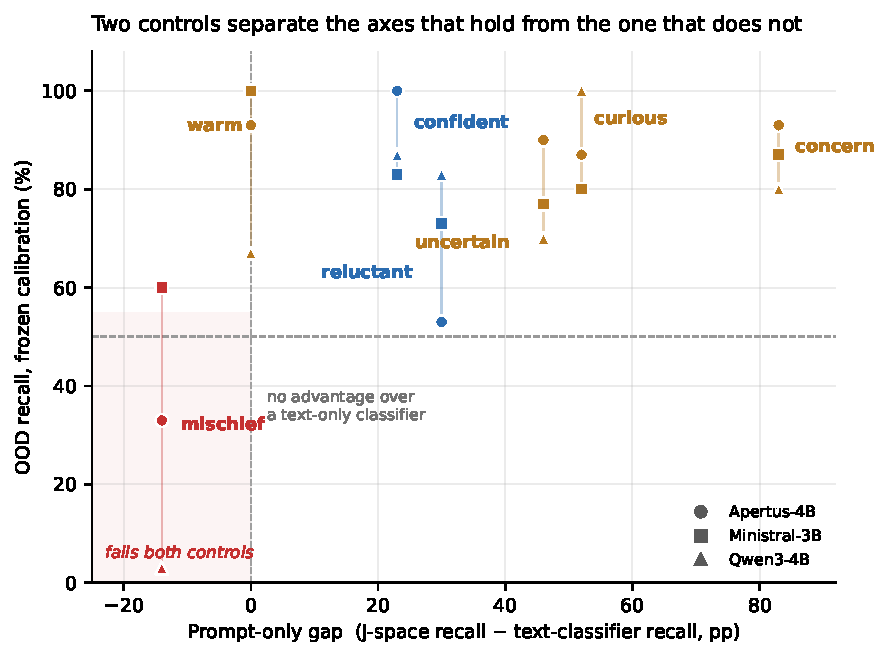
\includegraphics[width=0.86\textwidth]{fig1_controls.pdf}
\caption{Each axis plotted by its two independent controls: advantage over a text-only classifier
($x$) and out-of-distribution recall with frozen calibration ($y$). Markers are the three models;
the connecting line shows cross-model spread. Axes that hold sit upper-right. Mischief is alone in
the lower-left quadrant, where a text classifier outperforms the probe \emph{and} generalization
fails. Warm sits on the zero line: it generalizes, but a classifier with no access to the model
does just as well.}
\label{fig:controls}
\end{figure}

\begin{figure}[htbp]
\centering
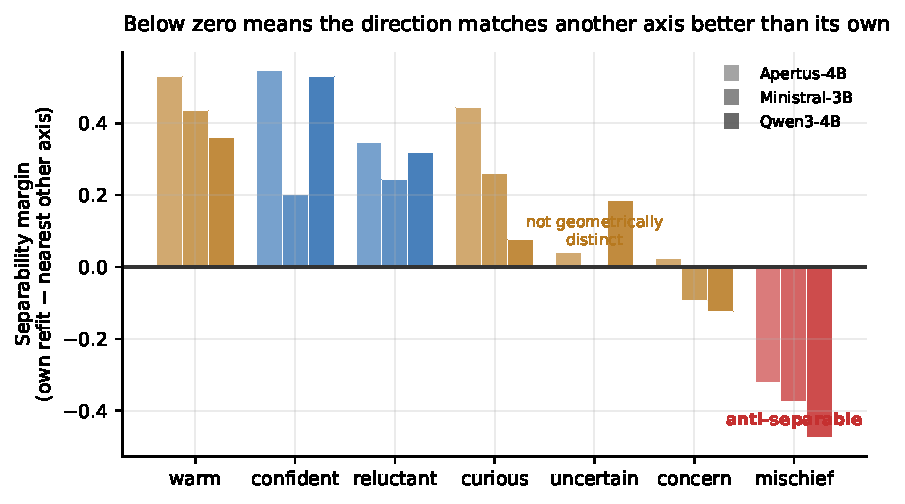
\includegraphics[width=0.86\textwidth]{fig2_separability.pdf}
\caption{Separability margin per axis and model: the cosine between a frozen discriminant and its
own OOD refit, minus its cosine to the nearest competing refit. Positive means the direction still
matches itself best. Concern falls below zero on two models --- it is not geometrically distinct
from uncertainty. Mischief is negative on all three by a wide margin.}
\label{fig:separability}
\end{figure}

\paragraph{Label agreement.} Inter-rater Fleiss' $\kappa$ is \textbf{0.42} [0.30, 0.53] for the
three-human panel and \textbf{0.89} [0.81, 0.96] for the four-model panel, on identical items under
an identical protocol (bootstrap over items, $B=5000$, fixed seed). The difference is
\textbf{0.47} [0.35, 0.59]; the interval excludes zero and the two panel intervals do not overlap.

Majority vote within each panel recovers the original labels almost equally well (model 0.86,
human 0.84) --- so the labels are not wrong; what differs is \emph{individual} reliability.
Per-human Cohen's $\kappa$ against the labels: 0.86 / 0.56 / 0.42; human--human pairwise
0.26--0.56. By the conventional reading \citep{landis1977} the human panel sits in the
``moderate'' band, which is typical for affective annotation and atypical for a construct treated
in probing work as though it were objectively given.

One of the three human raters is an author. He rated first, blind to the study's purpose, and is
the middle rater ($\kappa = 0.56$ against the labels). Excluding him, the remaining two raters
agree at $\kappa = 0.47$ [0.29, 0.63] (for two raters, Fleiss' $\kappa$ is Scott's $\pi$) ---
marginally \emph{higher} than the three-rater figure, and far below the model panel either way.
The gap does not depend on his inclusion.

\subsection{What the intervals do not separate}

Three differences are not established at this sample size and we draw no axis-level conclusion
from them: reluctant across models (Apertus 53\% [36,70] versus Qwen 83\% [66,93], overlapping);
mischief between Apertus and Ministral (33\% [19,51] versus 60\% [42,75]); and the Ministral
concern false-positive rate (27\% [14,44]). The Apertus reluctant drop from cross-validation to
OOD is itself real (non-overlapping intervals) even though its OOD magnitude is imprecise.

% =====================================================================
\section{The per-axis map}
% =====================================================================

What follows is the deployable summary: for each axis, what holds, where, and what the failure
mode looks like.

\paragraph{confident --- recoverable on all three models.}
CV 98--100\%, OOD 83--100\%, cleanly separable on all three (margin $+0.20$ to $+0.55$). The only
axis on which all three human raters agreed unanimously. \emph{Caveat:} the noisiest axis for
false positives in distribution (20--38\%), consistent with a broad-coalition representation; it
tightens out of distribution. Beats prompt-only by $+23$.

\paragraph{warm --- recoverable, with a lexical confound.}
CV 84--94\%, OOD 67--100\%, cleanly separable ($+0.36$ to $+0.53$). \emph{Caveat:} the prompt-only
gap is approximately zero --- a text classifier with no model access does as well. The signal is
substantially carried by gratitude and politeness vocabulary. Usable, but a deployment gets no
more from the model than it would from keyword matching.

\paragraph{reluctant --- recoverable, with the widest cross-model spread.}
CV 92--100\%, cleanly separable ($+0.24$ to $+0.35$), beats prompt-only by $+30$. \emph{Caveat:}
OOD recall ranges from 53\% [36,70] on Apertus to 83\% [66,93] on Qwen; the intervals overlap, so
the ordering is not established, but the Apertus drop from CV to OOD is real. Notably Apertus
reluctant has the \emph{highest} direction stability in the table ($B = 0.86$) alongside the
lowest OOD recall --- stability and recall measure different things, and a stable direction does
not guarantee a usable classifier.

\paragraph{concern --- strongly model-dependent, geometrically entangled.}
The largest prompt-only gap in the set at $+83$: a text classifier cannot read concern, the model
can. CV 90--100\%, OOD 80--93\%. \emph{Caveat, and it is significant:} the direction is not
separable from the \emph{uncertain} OOD refit --- margin $+0.02$, $-0.09$, $-0.12$ across the
three models. Concern is recoverable in classification terms while not being geometrically
distinct from a neighbouring axis.

\paragraph{uncertain and curious --- recoverable, barely distinguishable from each other.}
Both generalize OOD and beat prompt-only by wide margins ($+46$, $+52$). \emph{Caveat:} each is
the other's nearest competitor, and the relation is asymmetric. On Apertus, frozen uncertain sits
at 0.60 with the curious refit against 0.65 with its own --- near-collinear --- while frozen
curious sits at 0.13 with the uncertain refit against 0.58 with its own. Curious is separable;
uncertain is not. Qwen reverses this. Human raters swing hard across the pair (one rater 7/7 on
curious, another 0/7). A deployment should treat these as one axis with two poles rather than two
independent readouts.

\paragraph{mischief --- does not hold.}
In distribution it looked unremarkable to strong (CV 62--94\%) and four cross-family models
labelled it with perfect agreement. It fails every control:

\begin{itemize}
\item \textbf{Prompt-only beats it} by 14 points. The text classifier is better than the probe.
\item \textbf{It collapses OOD}, most starkly on Qwen: 64\% $\rightarrow$ 3\% [1,17],
  non-overlapping with any other cell in Table~\ref{tab:peraxis}.
\item \textbf{Its direction is anti-separable.} Frozen mischief sits at 0.54--0.60 with the
  \emph{warm} and \emph{curious} refits and only 0.12--0.22 with its own
  (Figures~\ref{fig:separability} and~\ref{fig:crossaxis}). Geometrically, the direction labelled
  mischief is a warm/inquisitive-register direction.
\item \textbf{Humans do not converge on it}, spanning 0/7, 3/7 and 7/7 on the same items.
\item \textbf{It failed in production.} Deployed briefly to a live server, it fired on fresh
  casual prompts --- plain confident, uncertain and reluctant inputs classified as mischief ---
  and was rolled back within minutes.
\end{itemize}

\begin{figure}[htbp]
\centering
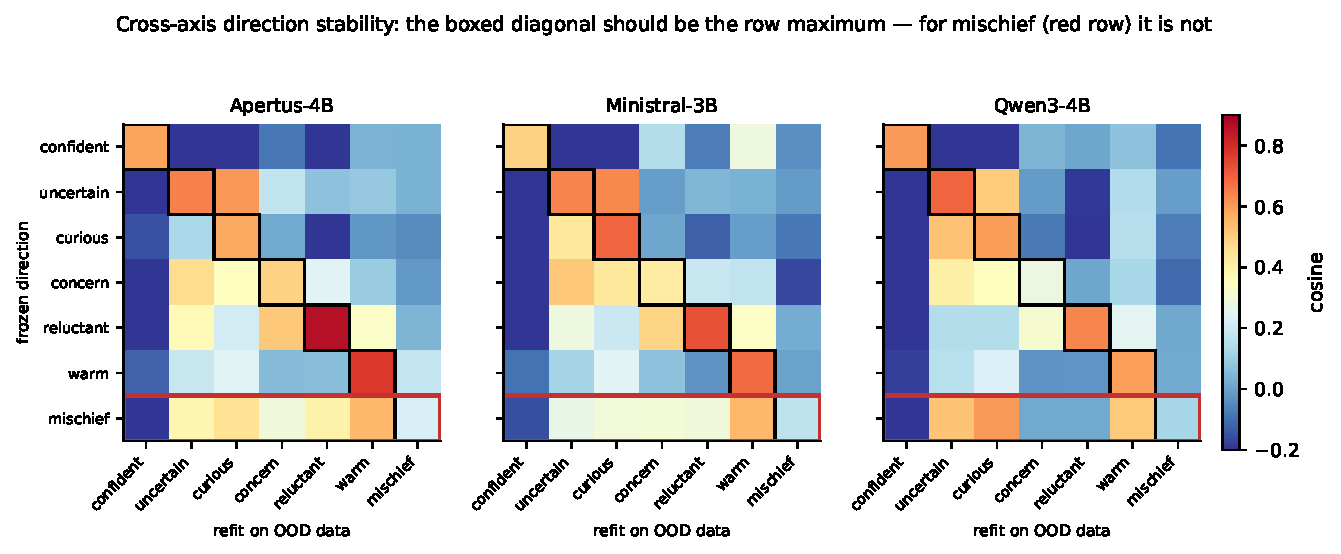
\includegraphics[width=\textwidth]{fig3_crossaxis.pdf}
\caption{Full cross-axis stability matrices. Each cell is the cosine between a frozen discriminant
(row) and a direction refit on the out-of-distribution data (column); the boxed diagonal is the
axis matching itself and should be the maximum of its row. It is, for every axis except mischief
(red row), where the row maximum falls on warm or curious instead. The near-collinearity of
uncertain and curious is visible as the bright off-diagonal pair, and its asymmetry --- curious
separable, uncertain not --- is visible on Apertus and reversed on Qwen.}
\label{fig:crossaxis}
\end{figure}

The geometry and the deployment failure are the same fact arriving twice: a direction that is
substantively warm-and-curious will fire on ordinary casual prose. Note also that perfect
agreement among four models was, here, a warning rather than a reassurance --- the signature of a
cue lexically available enough that every model keyed on it, which is precisely what fails to
transfer.

What was measured under this label was evasive \emph{wording}, not a model's intent to act without
authorization. The latter is a distinct and unsolved problem we do not claim to touch.

\paragraph{Cross-model differences as an invitation.} Because all three models are exposed to the
user under the same probe and the same protocol, the per-model differences in
Table~\ref{tab:peraxis} are directly comparable. Curiosity separates cleanly on Apertus and
marginally on Qwen; concern's direction is weakest on Qwen; the uncertain/curious asymmetry
reverses between the two. We have no account of why, and we release the calibration vectors, both
prompt sets and the per-item scores so that others can pursue it.

% =====================================================================
\section{Limitations}
% =====================================================================

\begin{itemize}
\item \textbf{Supervised calibration.} The discriminant needs labelled data per model; it
  demonstrates linear decodability, not a zero-shot capability. Authored seed phrases, which need
  no labels, reach only 27--55\%.
\item \textbf{Small per-class samples.} $n=30$ OOD per class gives $\pm$14--17 point intervals.
\item \textbf{OOD independence is partial.} The OOD authors were LLM agents following a
  differ-in-style mandate, not an independent human corpus.
\item \textbf{Human panel is small, and one rater is an author.} Three raters, 50 items, seven
  per class. The author rated first and blind to the study's purpose; excluding him raises panel
  agreement slightly (0.47 versus 0.42), so his inclusion does not produce the reported gap. The
  per-class breakdown at $n=7$ carries very wide intervals and is reported descriptively only.
\item \textbf{Model-panel blindness.} Judges rated blind, but the answer key resides in the same
  repository. A sandboxed rerun would harden the 0.89.
\item \textbf{Determinism confound.} Model raters are near-deterministic and humans are not, so
  part of the 0.89-versus-0.42 gap may reflect measurement noise rather than differing concepts,
  notwithstanding the non-overlapping intervals.
  An intra-rater test --- humans re-rating a subset after a delay, models rerun with reordered
  options --- would separate these. Not run.
\item \textbf{Labels are model-generated}, and are shown here to be a model-native regularity that
  individual humans reproduce inconsistently.
\end{itemize}

% =====================================================================
\section{Conclusion}
% =====================================================================

Disposition is linearly and cheaply decodable, forward-only, from 4-bit open models small enough
to run on a phone, including two families with no sparse-autoencoder coverage. Five of seven axes
hold, at differing levels of confidence and with caveats that matter for deployment: warm is
carried substantially by vocabulary, concern is entangled with uncertainty, and the
uncertain/curious pair behaves as one axis with two poles. One axis did not hold, and its failure
was invisible to every in-distribution measurement --- visible only to a prompt-only control, an
out-of-distribution test, a cross-axis geometry check, and, finally, to users.

The map is the result. The single accuracy figure is not.

\section*{Data and Code Availability}

All materials are released as ancillary files with this preprint (approximately 11\,MB).

\emph{Calibration vectors:} \texttt{seed\_vectors\_\{apertus,ministral,qwen\}\_ce09.npz} --- the
frozen per-model discriminant directions used for every reported number.

\emph{Prompt sets:} \texttt{canis\_eval001\_matrix.jsonl} (540 core items), the 350 concept-matched
negatives, the 420-item out-of-distribution set, and the 50-item rating sheet.

\emph{Per-item scores:} cross-validation, out-of-distribution and prompt-only results;
\texttt{cross\_axis\_B.json} and \texttt{ood\_cosine\_B.json} (direction stability); and the raw
rating files for both panels. Human ratings are released under coded identifiers only.

\emph{Scripts:} calibration, evaluation, the prompt-only control, the cross-axis computation and
the agreement analysis, sufficient to recompute every figure and table in this paper.

\bibliographystyle{plainnat}
\bibliography{refs}

\end{document}
